%**********************************************************
% Course IFJ @ FIT VUT Brno, 2017
% IFJ17 Project Compiler
%
% Authors:
% Erik Kelemen    - xkelem01
% Attila Lakatoš  - xlakat01
% Patrik Šober    - xsober00
% Tomáš Zubrik    - xzubri00
%**********************************************************

%******************* Dokumentacia *************************

\documentclass[a4paper, 12pt]{article}

\usepackage[left=2cm,text={17cm, 24cm},top=3cm]{geometry}
\usepackage[czech]{babel}
\usepackage[utf8]{inputenc}
\usepackage[IL2]{fontenc}
%\usepackage{times}
\usepackage{graphics}
\usepackage{url}
% Požadavky automatu
\usepackage{pgf}
\usepackage{tikz}
\usetikzlibrary{arrows,automata}
% Požadavky tabulky
\usepackage{diagbox}
% Rotace stránky
\usepackage{pdflscape}
% Citace
\usepackage{etoolbox}
\patchcmd{\thebibliography}{\section*{\refname}}{}{}{}

\pagenumbering{arabic}
\providecommand{\uv}[1]{\quotedblbase #1\textquotedblleft}
\interlinepenalty 10000 %nezalamovat odstavce

\begin{document}

%               Uvodna strana
%*******************************************************************************
\begin{titlepage}

\begin{center}
\fontsize{25}{20}\selectfont{\textsc{Vysoké učení technické v~Brně}}\\
\vspace{\stretch{0.0075}}
\fontsize{21}{0}\textsc{\selectfont{Fakulta informačních technologií}}\\
\vspace{\stretch{0.15}}
%Logo
\begin{figure}[ht]
    \begin{center}
        \scalebox{0.6}{
\includegraphics{fit_logo.png}}
    \end{center}
\end{figure}

\vspace{\stretch{0.2}}
\LARGE{Dokumentácia k projektu do predmetu IFJ a IAL}\\
\Large{Implementácia prekladača jazyka IFJ17}\\ 
\bigskip
\Large{Tím \textit{126}, varianta \textit{II}}\\
\Large{Rozšírenia BOOLOP, BASE}
\vspace{\stretch{0.618}}
\end{center}

\begin{center}
\begin{large}
\begin{tabbing}
Skip   : \quad \quad \= XXXXXXX XXXX \quad \= xposto02 \quad \= 25 \%\kill
       Vedúci:  \> Kelemen Erik \> xkelem01 \> 25 \% \\
   		     	\> Lakatoš Attila  \> xlakat01 \> 25 \% \\
                \> Šober Patrik  \> xsober00 \> 25 \% \\
                \> Zubrik Tomáš \> xzubri00 \> 25 \% \\
\end{tabbing}
\end{large}
\end{center}

\end{titlepage}


%                   Obsah
%*******************************************************************************
\tableofcontents
\newpage

%                   Úvod
%*******************************************************************************
\section{Úvod} \label{uvod}

Dokumentácia k projektu popisuje implementáciu prekladača, ktorý načíta zdrojový kód v jazyku IFJ17, ktorý je zjednodušenou podmnožinou jazyka FreeBasic a prevedie preklad na cieľový kód jazyka IFJcode17, ktorý je ďalej interpretovateľný. Prekladač sa skladá z nasledujúcich 3 fundamentálnych častí:

\begin{itemize}
	\item Lexikálny analyzátor
	\item Syntaktický analyzátor
	\item Sémantický analyzátor
\end{itemize}

%                   Úlohy v~tíme a~rozdelenie práce
%*******************************************************************************
\section{Úlohy v~tíme a~rozdelenie práce} \label{team}

\subsection{Rozdelenie úloh na jednotlivých častiach projektu}
\begin{itemize}
	\item Kelemen Erik -- syntaktický analyzátor, tabuľka symbolov
	\item Lakatoš Attila -- spracovanie výrazov, generovanie kódu
	\item Šober Patrik -- lexikálny analyzátor, testovanie
	\item Zubrik Tomáš -- sémantický analyzátor, dokumentácia

\end{itemize}

\subsection{Priebeh}
Tímový projekt takýchto rozmerov prináša nové problémy, ale zároveň dokáže prispieť k~našim skúsenostiam. Ako štvorčlenný tím sme si na začiatku spolupráce museli zvoliť vhodný komunikačný kanál a~verzovací systém. 
Ako komunikačný kanál sme použili sociálnu sieť \texttt{facebook}. 
Ako verzovací systém sa rozhodli využiť \texttt{git} prostredníctvom webovej služby \texttt{GitHub}, kde vedúci tímu založil privátny repozitár, ktorý sme využili pre naše potreby. 
Určili sme taktiež základné konvencie pre písanie kódu. 

Problémy a pripomienky sme riešili cez sociálnu sieť, v prípade nutnosti sme zorganizovali stretnutie vo vopred dohodnutom čase a na dohodnutom mieste. Jednotlivé časti boli implementované súčasne a každý na svojej časti pracoval s pomocou ostatných. S prípadnými otázkami a nejasnosťami sa člen tímu obrátil na vedúceho tímu. Pre testovanie sme využili automatické testy, ktoré boli implementované ako \texttt{shell script}.  

\newpage

\section{Implementáca prekladača jazyka IFJ17} \label{implementace}



%                   Lexikalna analyza
%*******************************************************************************
\subsection{Lexikálna analýza} \label{lexer}

Lexikálny analyzátor je fundamentálnou a nevyhnutnou časťou prekladača. Je založený na deterministickom konečnom automate a jeho hlavnou úlohou je čítať zdrojový kód a na základe lexikálnych pravidiel daného jazyka rozdeliť jednotlivé postupnosti znakov na príslušné lexikálne jednotky -- lexémy.

Lexikálne jednotky sú v programe reprezentované ako tokeny, teda zdrojový kód chápeme ako konečnú postupnosť tokenov. Každý token obsahuje dáta o jeho type, prípadne reťazec alebo číselnú hodnotu. Dáta do tokenov sú zapisované pomocou nami implementovaných funkcií v hlavičkovom súbore \texttt{string.h}.

Lexikálna analýza ignoruje všetky biele znaky, vrátane medzier, tabulátorov a komentárov, ktoré nie sú podstatné pre programový tok. Zdrojový kód môže obsahovať 2 typy komentárov: 
Riadkový komentár, ktorý sa začína znakom \texttt{'} a končí na konci riadku. 
Blokový komentár ktorý je ohraničený sekvenciou znakov \texttt{/'} a \texttt{'/}. Obidva typy komentárov môžu byť umiestnené kdekoľvek v programe.

Po spustení prekladu vytvorí lexikálny analyzátor dané tokeny s príslušnými dátami a uloží ich do zásobníka tokenov, s ktorým ďalej pracuje syntaktický analyzátor. Princíp fungovania lexikálnej analýzy reprezentuje deterministický konečný automat v prílohe \ref{subsec:automat}.


%                   Syntaktická a sémantická analýza
%*******************************************************************************
\subsection{Syntaktická a sémantická analýza} \label{parser}
Syntaktický a sémantický analyzátor predstavuje najdôležitejšiu a najzlozitejšiu časť našej implementácie. Riadenie v programe preberá po lexikálnej analýze a riadi tok programu až k úplnému spracovaniu zdrojového kódu.

\subsubsection{Spracovanie jazykových konštrukcií}
Syntaktická analýza je implementovaná rekurzívnym zostupom a je riadená na základe vytvorenej LL-gramatiky v prílohe \ref{subsec:llgram}. Neterminály predstavujú v našej implementácii funkcie, ktoré sú volané v závislosti od nasledujúceho tokenu. Syntakticky správne napísaný zdrojový kód musí podliehať LL-gramatike, len v tom prípade je syntaktická analýza úspešná.
Spolu so syntaktickou analýzou sú súčasne vykonávané sémantické kontroly. Pri deklarácii a definícii funkcie alebo premennej je daný identifikátor uložený do príslušnej tabuľky symbolov. Funkcie sú uložené do globálnej tabuľky symbolov, premenné zas do lokálnych tabuliek symbolov jednotlivých funkcií a hlavného tela programu. 

Pri spracovaní tela funkcií a hlavného tela programu sa zároveň generujú príslušné inštrukcie, ktoré sú pripojené do výstupného reťazca, reprezentujúceho inštrukčnú pásku.

Ak sa behom syntaktickej analýzy narazí na výraz, je riadenie programu predané precedenčnej syntaktickej analýze pre spracovanie výrazov. Po spracovaní výrazu a vygenerovaní príslušných inštrukcií sa riadenie programu znovu vráti syntaktickej analýze.

Po spracovaní celého zdrojového súboru sa prevádzajú záverečné sémantické kontroly. Kontroluje sa definovanosť všetkých funkcií a prebehne kontrola či sa hlavné telo programu začinajúce kľúčovým slovom \texttt{SCOPE} vyskytuje v zdrojovom kóde len raz apod.

Po dokončení záverečných sémantických kontrol je syntaktická a~sémantická analýza ukončená a~na~štandardný výstup sa výpiše celá inštrukčná páska, ktorú spracuje interpret.

\newpage

\subsubsection{Spracovanie výrazov}

Spracovanie výrazu sa prevedie vtedy, ak podľa LL-gramatiky nasleduje neterminál \texttt{E}, ktorý reprezentuje výraz. Spracovanie výrazov je riadené precedenčnou tabuľkou uvedenou v prílohe \ref{subsec:precetable}.
Spracovanie výrazu prebieha v 3 krokoch. Najprv sa kontroluje sémantika jednotlivých premenných a prevedie sa syntaktická kontrola, či ide o prípustný zápis výrazu. V druhom kroku sa prevedie výraz z infixového zápisu na postfixový pomocou zásobníka. V treťom kroku je vyhodnotený a vyčíslený postfixový výraz, prípadne sú uskutočnené implicitné konverzie a následne sú vygenerované príslušné inštrukcie, ktoré sú pripojené do výstupného reťazca, reprezentujúceho inštrukčnú pásku.

Pri neúspešnom spracovaní výrazu je preklad ukončený a program je ukončený s návratovou hodnotou podľa konvencie reprezentujúci príslušnú chybu.

\subsubsection{Volanie funkcií}

Volanie funkcií spracúva syntaktická analýza. Kontrolujú sa návratové typy funkcií a premenných do ktorých je funkcia priradená a taktiež typy a počet parametrov, s prípadnými implicitnými konverziami. Pred zavolaním funkcie sú jej parametre uložené na dočasný rámec, ktorý sa v ďalšom kroku pridá na lokálny zásobník rámcov. Následne sa prevádzajú inštrukcie v tele funkcie. Pri návrate z funkcie sa jej návratová hodnota uloží do vyhradenej premennej \texttt{\%returnval} a je pridaná na vrchol dátového zásobníka interpretu pre následné priradenie do premennej. Inštrukcie sú ďalej vykonávané od miesta, kde bola funkcia zavolaná.

\subsubsection{Vstavané funkcie}
Dôležitou súčasťou sú vstavané funkcie. Na začiatku prekladu sa do výstupného reťazca, reprezentujúceho inštrukčnú pásku pripoja inštrukcie pre všetky vstavané funkcie a taktiež sa jednotlivé funkcie ako položky uložia do globálnej tabuľky symbolov. Pri následnom volaní vstavanej funkcie ide o klasické volanie funkcie. 

%                   Interpret
%*******************************************************************************
\bigskip
\bigskip
\subsection{Použitie interpretu} \label{interpret}

K dispozícii sme mali instrukčnú sadu. Našou úlohou nebolo interpret implementovať, ale správne skonštruovať prípustné inštrukcie z inštrukčnej sady, ktoré budú interpretovateľné a po ich prevedení sa dostaneme k správnemu výsledku.

\newpage

%                   Pouzite datove struktury
%*******************************************************************************
\subsection{Použité datové štruktúry} \label{datastructs}

\subsubsection{Tabuľka s rozptýlenými položkami}
Pre implementáciu tabuľky symbolov sme zvolili variantu \textit{II.} - tabuľku s rozptýlenými položkami. Dôležitý faktor tvorí rýchlosť vyhľadávania jednotlivých položiek. Položka obsahuje kľúč, z ktorého sa vypočíta príslušný index v tabuľke, dôležité dáta o položke a ukazateľ na ďalšiu položku. Položky na tom istom indexe v tabuľke sú prepojené ukazateľmi a tvoria jednosmerný explicitne viazaný lineárny zoznam. Ako rozptyľovaciu funkciu sme zvolili vhodnú variantu pre reťazce.

\subsubsection{Zásobník}
Zásobník je dynamická datová štruktúra, ktorá umožňuje pracovať s položkou na vrchole zásobníka. Zásobník sme použili pri spracovaní výrazov, konkrétne pri prevode z infixového zápisu na postfixový a pri ich vyčíslovaní.  

\subsubsection{Reťazec}
Reťazec je v podstate dynamické pole znakov alebo vektor. V našej implementácii táto štruktúra obsahuje konkrétny reťazec, jeho dĺžku a kapacitu nutnú pre jeho alokáciu v pamäti. V prípade potreby sa zvýši kapacita alokovaného reťazca.

\subsubsection{Dynamické pole}
Dynamické pole je dátová štruktúra, ktorá sa využíva ak vopred nie je známy presný počet položiek. Dynamické pole sme využili pre implementáciu zásobníka tokenov, ktorý sa po spustení programu naplní ukazateľmi na tokeny a je možné s nimi ďalej pracovať.

\bigskip
\bigskip
\subsection{Rozšírenia} \label{extensions}
Implementované rozšírenia v našom projekte sú BOOLOP a BASE. Rozšírenie BASE spočívalo v pridaní nových stavov príslušiacich pre dvojkové, osmičkové a šestnástkové čísla. Následne sme implementovali funkciu na konverziu daného typu čísla na integer. Rozšírenie BOOLOP spočívalo v priadaní nových elementov - operátorov do precedenčnej tabuľky a následnej implementácii, ktorá sa prejavila hlavne v precedenčnej syntaktickej analýze.

\newpage

%                   Prílohy
%*******************************************************************************
\section{Prílohy} \label{prilohy}

\renewcommand\thesubsection{\thesection.\Alph{subsection}}

%************************ FSM **************************
\subsection{Diagram konečného automatu lexikálnej analýzy \cite{automata}} \label{subsec:automat}
\begin{figure}[ht]
    \begin{center}
        \scalebox{0.35}{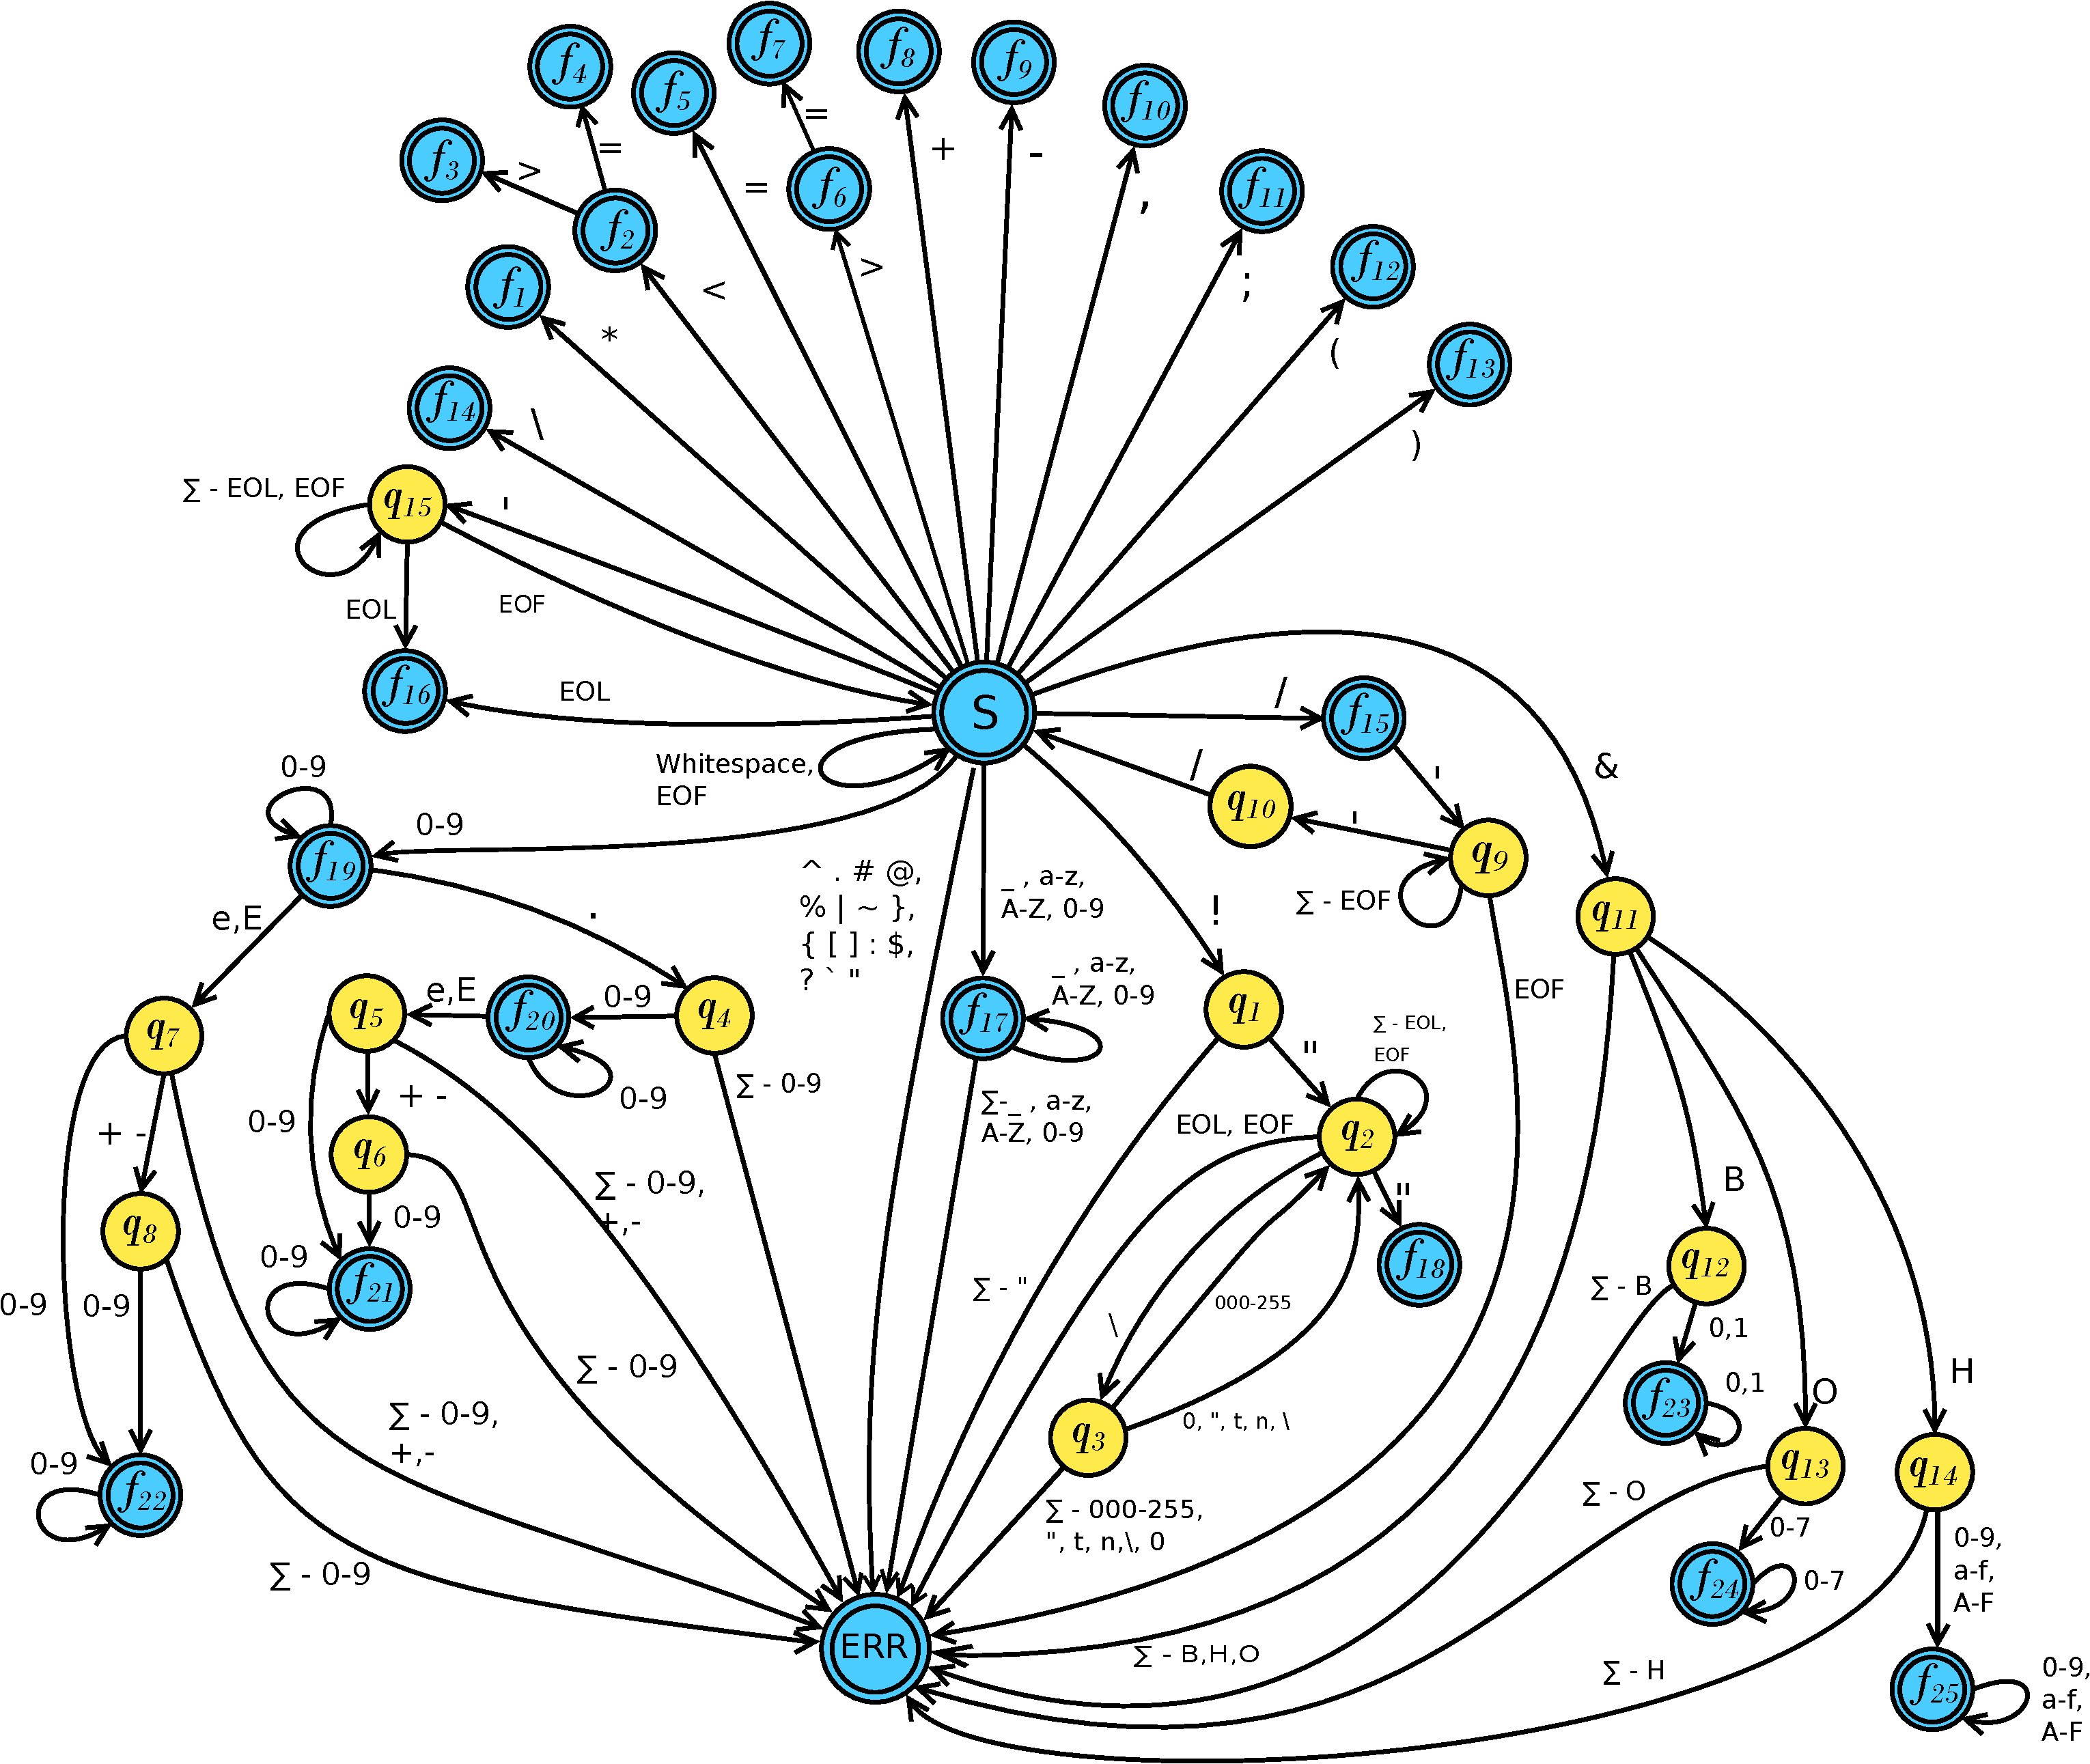
\includegraphics{fsm.pdf}}
    \end{center}
\end{figure}

\begin{table}[ht]
{
	\renewcommand{\arraystretch}{1.3}
	\begin{center}
		\catcode`\-=12
		\begin{tabular}{| c | l | c | l |} 
		\hline
		\textbf{Označení}  & \textbf{Název stavu}    & \textbf{Označení}  & \textbf{Název stavu}  \\ \hline
		q\textsubscript{1} & EXCLAMATION\_MARK       & q\textsubscript{10} & BLOCK\_COMMENT\_END  \\ \hline
		q\textsubscript{2} & STRING\_LITERAL\_BEGINS & q\textsubscript{11} & BASE             	  \\ \hline
		q\textsubscript{3} & ESCAPE\_SEQUENCE        & q\textsubscript{12} & BINARY\_START		  \\ \hline
		q\textsubscript{4} & DOUBLE\_1               & q\textsubscript{13} & OCTAL\_START		  \\ \hline
		q\textsubscript{5} & DOUBLE\_2               & q\textsubscript{14} & HEX\_START		      \\ \hline
		q\textsubscript{6} & DOUBLE\_3               & q\textsubscript{15} & LINE\_COMMENT        \\ \hline
		q\textsubscript{7} & INT\_EXP\_1 	         & 											  \\ \hline
		q\textsubscript{8} & INT\_EXP\_2 			 & 					   & 					  \\ \hline
		q\textsubscript{9} & BLOCK\_COMMENT\_START   & 					   & 					  \\ \hline
		\end{tabular}
	\caption{Konečný automat lexikálneho analyzátora - Stavy}	
	\end{center}
}  
\end{table}
\begin{table}[!ht]
{
	\renewcommand{\arraystretch}{1.3}
	\begin{center}
		\catcode`\-=12
		\begin{tabular}{| c | l | c | l |} 
		\hline
		\textbf{Označení}   & \textbf{Název stavu}             & \textbf{Označení}   & \textbf{Název stavu}  \\ \hline
		S                   & START, EOF                       & f\textsubscript{14} & DIV2     			 \\ \hline
		f\textsubscript{1}  & MUL                              & f\textsubscript{15} & DIV                   \\ \hline
		f\textsubscript{2}  & LESS\_THAN                       & f\textsubscript{16} & NEWLINE         		 \\ \hline
		f\textsubscript{3}  & NOT\_EQUAL                       & f\textsubscript{17} & IDENTIFICATOR   		 \\ \hline
		f\textsubscript{4}  & LESS\_OR\_EQUAL                  & f\textsubscript{18} & STRING\_LITERAL 		 \\ \hline
		f\textsubscript{5}  & EQUAL                            & f\textsubscript{19} & INTEGER         		 \\ \hline
		f\textsubscript{6}  & GREATER\_THAN                    & f\textsubscript{20} & DOUBLE          		 \\ \hline
		f\textsubscript{7}  & GREATER\_OR\_EQUALS              & f\textsubscript{21} & DOUBLE\_WITH\_EXP 	 \\ \hline
		f\textsubscript{8}  & ADD                              & f\textsubscript{22} & INT\_WITH\_EXP 		 \\ \hline
		f\textsubscript{9}  & SUB                              & f\textsubscript{23} & BIN\_NUM 			 \\ \hline
		f\textsubscript{10} & COMA                             & f\textsubscript{24} & 	OCTAL\_NUM	   		 \\ \hline
		f\textsubscript{11} & SEMICOLON                        & 			     	 & 			             \\ \hline
		f\textsubscript{12} & LEFT\_PARANTHESIS     		   & 			         & 	     				 \\ \hline
		f\textsubscript{13} & RIGHT\_PARANTHESIS    		   & 			         & 			 			 \\ \hline
		\end{tabular}
	\caption{Konečný automat lexikálneho analyzátora - Konečné stavy}	
	\end{center}
}  
\end{table}
\clearpage
\newpage

%**************** LL gramatika**********************
\subsection{LL-gramatika} \label{subsec:llgram}
\begin{verbatim}
START-> FUNBLOCK SCOPEBLOCK  
SCOPEBLOCK-> scope STATEMENTBLOCK end scope  
FUNBLOCK-> declare function id left FUNDECPARAMS right as TYPE eol FUNBLOCK  
FUNBLOCK-> function id left FUNDECPARAMS right as TYPE eol STATEMENTBLOCK
           end function eol FUNBLOCK  
FUNBLOCK-> eol FUNBLOCK  
FUNBLOCK-> epsilon  
FUNDECPARAMS-> id as TYPE FUNDECPARAMSNEXT  
FUNDECPARAMS-> epsilon
FUNDECPARAMSNEXT-> comma FUNDECPARAMS  
FUNDECPARAMSNEXT-> epsilon   
TYPE-> integer   
TYPE-> double   
TYPE-> string   
STATEMENTBLOCK-> DECORASSIGN STATEMENTBLOCK   
DECORASSIGN-> dim id as TYPE DECASSIGN eol   
DECASSIGN-> equal E   
DECASSIGN-> epsilon   
STATEMENTBLOCK-> FUNCALLORASSIGN STATEMENTBLOCK   
FUNCALLORASSIGN-> id equal FUNCALLORASSIGN2   
FUNCALLORASSIGN2-> id left FUNCALLPARAMS right eol   
FUNCALLORASSIGN2-> E eol   
FUNCALLPARAMS-> FUNCALLPARAM FUNCALLPARAMSNEXT   
FUNCALLPARAMS-> epsilon   
FUNCALLPARAM-> id   
FUNCALLPARAM-> CONSTVALUE   
FUNCALLPARAMSNEXT-> comma  FUNCALLPARAMS   
FUNCALLPARAMSNEXT-> epsilon   
CONSTVALUE-> integer_value   
CONSTVALUE-> double_value 
CONSTVALUE-> string_value   
STATEMENTBLOCK-> if E semicolon then eol STATEMENTBLOCK ELSESTATEMENT 
                 end if STATEMENTBLOCK   
ELSESTATEMENT-> else eol STATEMENTBLOCK   
ELSESTATEMENT-> epsilon  
STATEMENTBLOCK-> print E semicolon EXPRNEXT eol STATEMENTBLOCK   
EXPRNEXT-> E semicolon EXPRNEXT   
EXPRNEXT-> epsilon   
STATEMENTBLOCK-> input id eol STATEMENTBLOCK   
STATEMENTBLOCK-> do while E eol STATEMENTBLOCK loop STATEMENTBLOCK   
STATEMENTBLOCK-> return E   
STATEMENTBLOCK-> epsilon   
STATEMENTBLOCK-> eol STATEMENTBLOCK 
\end{verbatim}
\newpage

%********************LL tabulka***************************
\begin{landscape}
\begin{figure}[ht]
\subsection{LL-tabuľka} \label{subsec:lltable}
    \begin{center}
        \scalebox{0.9}{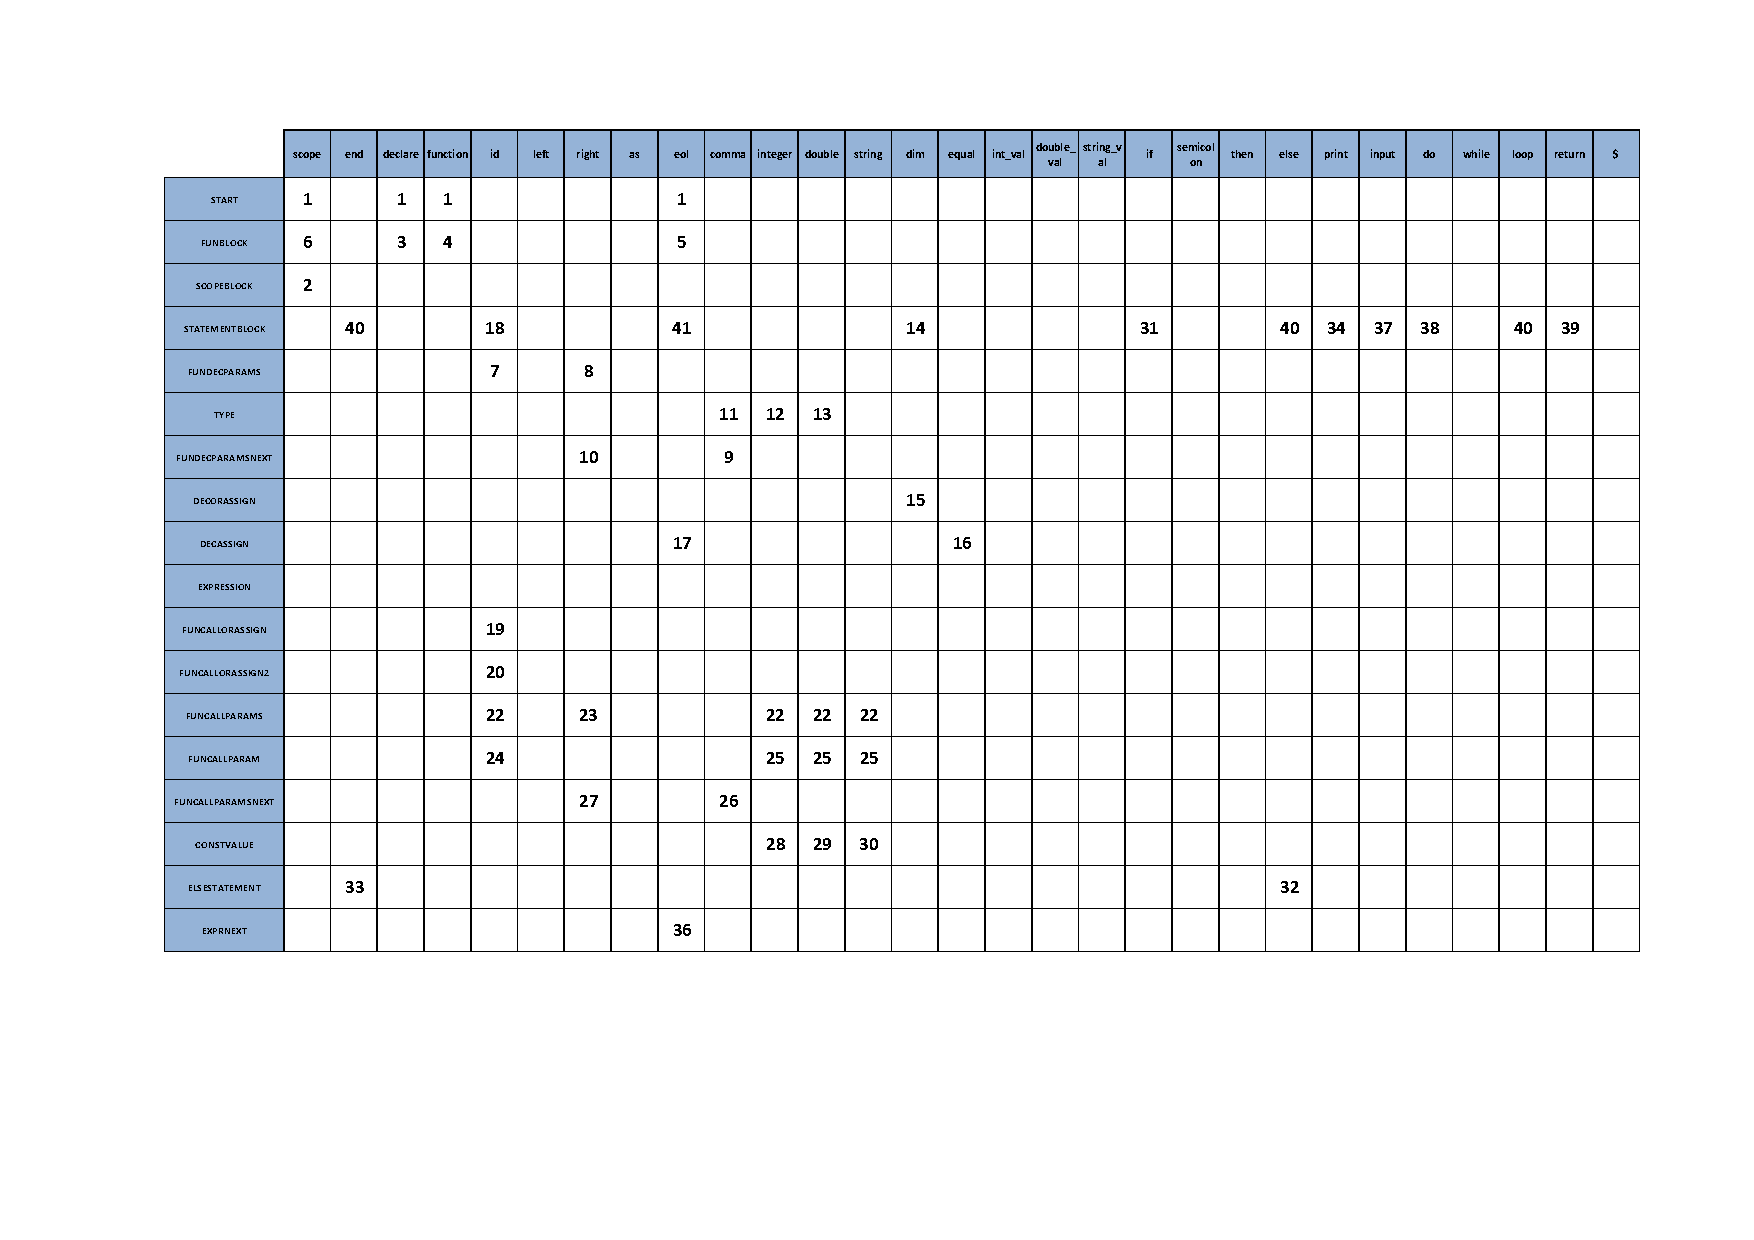
\includegraphics{lltable.pdf}}
    \end{center}
\end{figure}
\end{landscape}
\newpage


%**************Precedencna tabulka******************
\begin{landscape}
\begin{figure}[ht]
\subsection{Precedenčná tabuľka} \label{subsec:precetable}
    \begin{center}
        \scalebox{0.9}{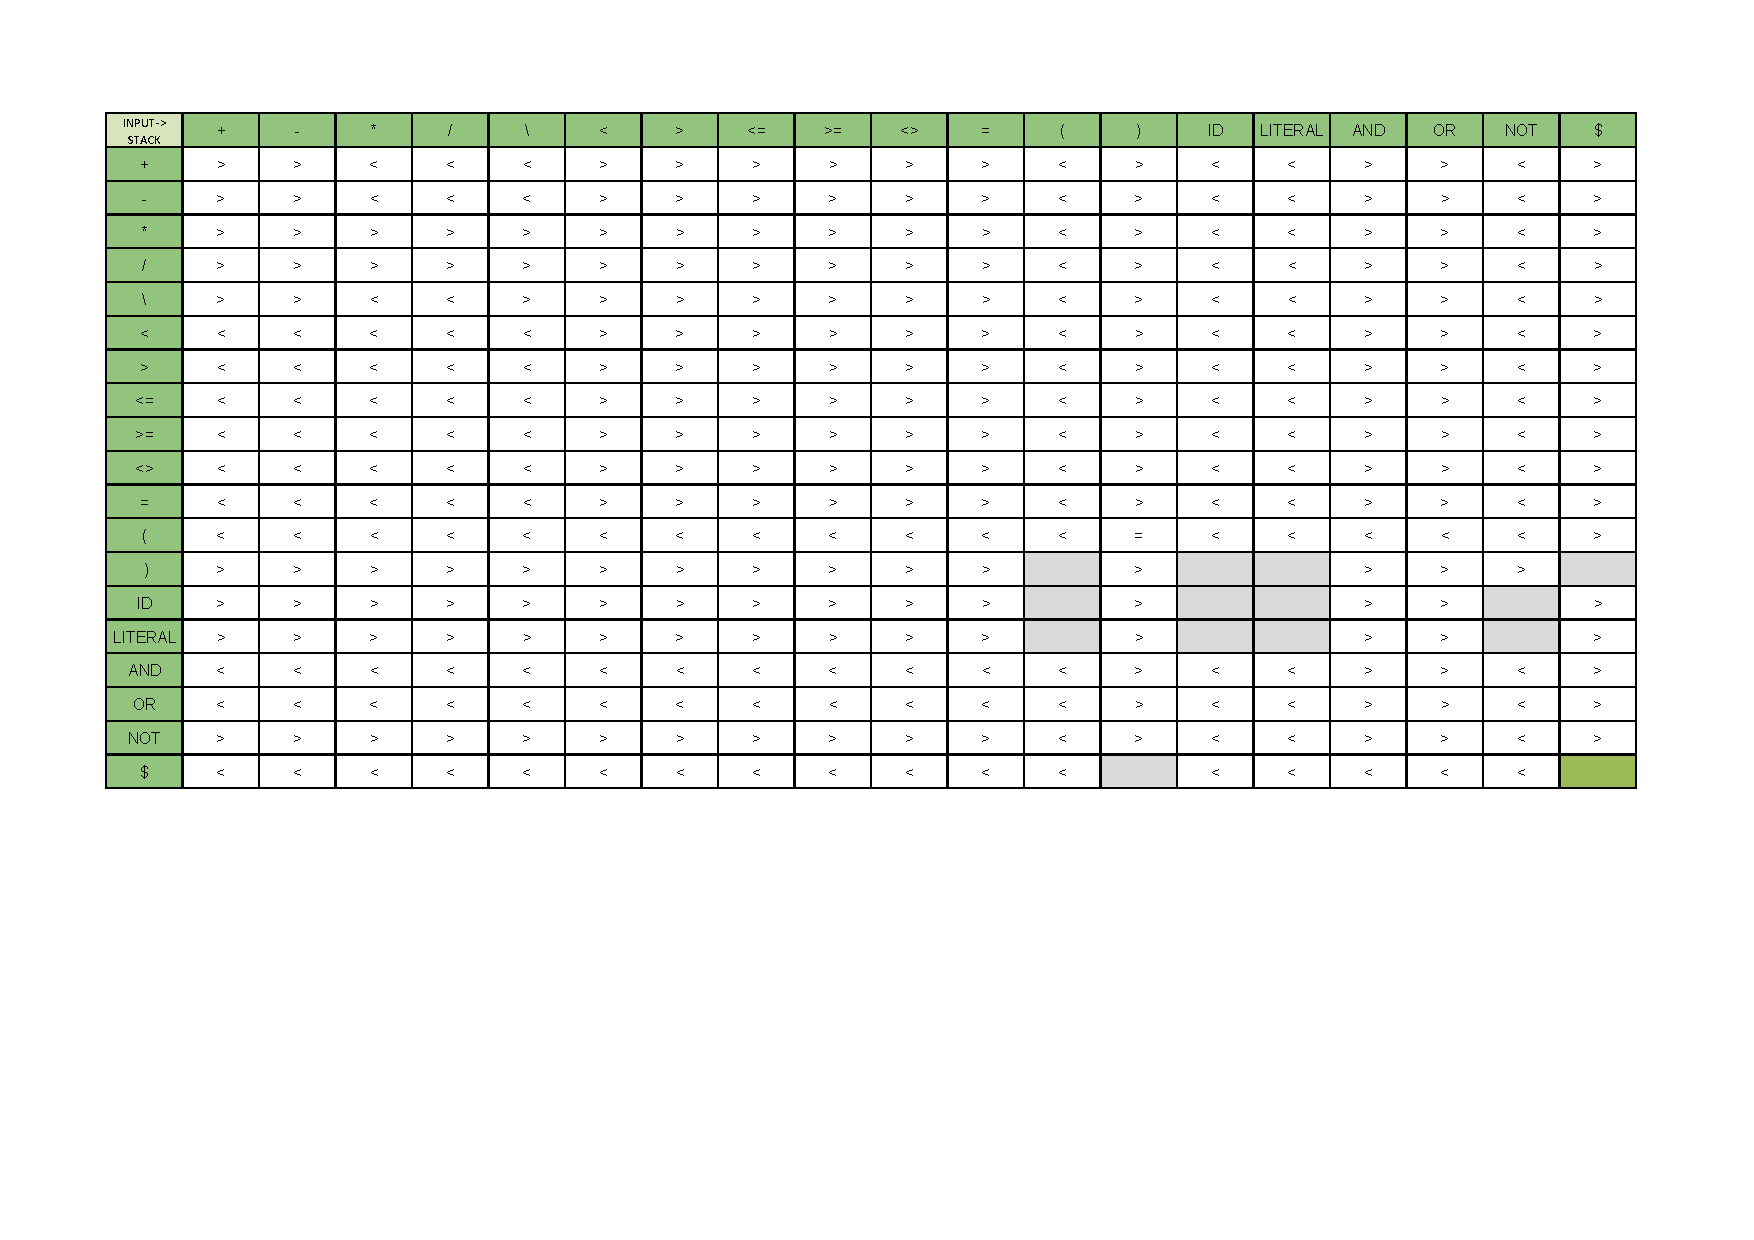
\includegraphics{prectab.pdf}}
    \end{center}
\end{figure}
\end{landscape}
\newpage

\section{Referencie} \label{reference}

\begin{thebibliography}{2}

\bibitem{automata} 
WALLACE, E.
\textit{Finite State Machine Designer}
[online]. 2010 [cit. 2015-12-13]. Dostupné na: \texttt{http://madebyevan.com/fsm/}

\bibitem{ial}
Prof. Ing. Jan Maxmilián Honzík, CSc.
\textit{Algoritmy IAL: Sudijní opora}
[online]. Verze 17R. 2017-12-3 [cit. 2017-12-5].
Dostupné na: \texttt{https://wis.fit.vutbr.cz/FIT/st/\\course-files-st.php/course/IAL-IT/texts/Opora-IAL-2017-verze-17-B.pdf}

\end{thebibliography}

\end{document}
